% Options for packages loaded elsewhere
\PassOptionsToPackage{unicode}{hyperref}
\PassOptionsToPackage{hyphens}{url}
%
\documentclass[
]{article}
\usepackage{amsmath,amssymb}
\usepackage{iftex}
\ifPDFTeX
  \usepackage[T1]{fontenc}
  \usepackage[utf8]{inputenc}
  \usepackage{textcomp} % provide euro and other symbols
\else % if luatex or xetex
  \usepackage{unicode-math} % this also loads fontspec
  \defaultfontfeatures{Scale=MatchLowercase}
  \defaultfontfeatures[\rmfamily]{Ligatures=TeX,Scale=1}
\fi
\usepackage{lmodern}
\ifPDFTeX\else
  % xetex/luatex font selection
\fi
% Use upquote if available, for straight quotes in verbatim environments
\IfFileExists{upquote.sty}{\usepackage{upquote}}{}
\IfFileExists{microtype.sty}{% use microtype if available
  \usepackage[]{microtype}
  \UseMicrotypeSet[protrusion]{basicmath} % disable protrusion for tt fonts
}{}
\makeatletter
\@ifundefined{KOMAClassName}{% if non-KOMA class
  \IfFileExists{parskip.sty}{%
    \usepackage{parskip}
  }{% else
    \setlength{\parindent}{0pt}
    \setlength{\parskip}{6pt plus 2pt minus 1pt}}
}{% if KOMA class
  \KOMAoptions{parskip=half}}
\makeatother
\usepackage{xcolor}
\usepackage[margin=1in]{geometry}
\usepackage{graphicx}
\makeatletter
\def\maxwidth{\ifdim\Gin@nat@width>\linewidth\linewidth\else\Gin@nat@width\fi}
\def\maxheight{\ifdim\Gin@nat@height>\textheight\textheight\else\Gin@nat@height\fi}
\makeatother
% Scale images if necessary, so that they will not overflow the page
% margins by default, and it is still possible to overwrite the defaults
% using explicit options in \includegraphics[width, height, ...]{}
\setkeys{Gin}{width=\maxwidth,height=\maxheight,keepaspectratio}
% Set default figure placement to htbp
\makeatletter
\def\fps@figure{htbp}
\makeatother
\setlength{\emergencystretch}{3em} % prevent overfull lines
\providecommand{\tightlist}{%
  \setlength{\itemsep}{0pt}\setlength{\parskip}{0pt}}
\setcounter{secnumdepth}{-\maxdimen} % remove section numbering
\usepackage[utf8]{inputenc}

\usepackage{setspace}
\doublespacing

\usepackage[version = 4]{mhchem}

% TABLES
\usepackage{tabularx}
\usepackage{threeparttable}
\usepackage{booktabs}
\usepackage{rotating}
\usepackage{csvsimple}

% SIUNITX
\usepackage{siunitx}

\sisetup{separate-uncertainty, multi-part-units = repeat}

\newcommand\SIci[4]{\SI{#1}{#2} ({95\%}CI: \SIrange{#3}{#4}{#2})} % Confidence interval
\newcommand\SIcv[1]{\SI{#1}{\percent}} % Coefficient of variation

\DeclareSIUnit[number-unit-product = {}]\degC{\degreeCelsius}
\DeclareSIUnit[number-unit-product = {}]\p{\percent}
\DeclareSIUnit[number-unit-product = \;]\s{\second}
\DeclareSIUnit[number-unit-product = \;]\min{\minute}
\DeclareSIUnit[number-unit-product = \;]\h{\hour}
\DeclareSIUnit[number-unit-product = \;]\d{\day}
\DeclareSIUnit[number-unit-product = \;]\mm{\milli\meter}
\DeclareSIUnit[number-unit-product = \;]\mL{\milli\liter}
\DeclareSIUnit[number-unit-product = \;]\L{\liter}
\DeclareSIUnit[number-unit-product = \;]\cubicm{\cubic\meter}
\DeclareSIUnit[number-unit-product = \;]\kg{\kilo\gram}
\DeclareSIUnit[number-unit-product = \;]\mg{\milli\gram}
\DeclareSIUnit[number-unit-product = \;]\mgL{\milli\gram\per\liter}
\DeclareSIUnit[number-unit-product = \;]\ug{\micro\gram}
\DeclareSIUnit[number-unit-product = \;]\ugL{\micro\gram\per\liter}
\DeclareSIUnit[number-unit-product = \;]\molL{\mole\per\liter}
\DeclareSIUnit[number-unit-product = \;]\mmolL{\milli\mole\per\liter}
\DeclareSIUnit[number-unit-product = \;]\gmol{\gram\per\mole}
\DeclareSIUnit[number-unit-product = \;]\mgkg{\milli\gram\per\kilo\gram}
\DeclareSIUnit[number-unit-product = \;]\gkg{\gram\per\kilo\gram}

% Symbols
\usepackage{amssymb}

% GLOSSARIES
\usepackage{glossaries}

\newacronym{adc}{ADC}{apparent digestibility coefficient}
\newacronym{atp}{ATP}{adenosine triphosphate}
\newacronym{cp}{CP}{crude protein}
\newacronym{cv}{CV}{coefficient of variation}
\newacronym{dna}{DNA}{desoxyribonucleic acid}
\newacronym{fr}{FR}{feeding rate}
\newacronym{mle}{MLE}{maximum likelihood estimation}
\newacronym{ras}{RAS}{recirculation aquaculture system}
\newacronym{rna}{RNA}{ribonucleic acid}
\newacronym{tan}{TAN}{total ammonia nitrogen}
\newacronym{tin}{TIN}{total inorganic nitrogen}
\ifLuaTeX
  \usepackage{selnolig}  % disable illegal ligatures
\fi
\IfFileExists{bookmark.sty}{\usepackage{bookmark}}{\usepackage{hyperref}}
\IfFileExists{xurl.sty}{\usepackage{xurl}}{} % add URL line breaks if available
\urlstyle{same}
\hypersetup{
  pdftitle={The nutrient budget of closed and semi-open aquaculture systems},
  pdfauthor={Anıl A. Tellbüscher},
  hidelinks,
  pdfcreator={LaTeX via pandoc}}

\title{The nutrient budget of closed and semi-open aquaculture systems}
\usepackage{etoolbox}
\makeatletter
\providecommand{\subtitle}[1]{% add subtitle to \maketitle
  \apptocmd{\@title}{\par {\large #1 \par}}{}{}
}
\makeatother
\subtitle{Assessment of contributions from different nutrient sources
based on permutation analysis}
\author{Anıl A. Tellbüscher}
\date{Last updated: 14.02.2024}

\begin{document}
\maketitle

\hypertarget{permutation-analysis}{%
\section{Permutation analysis}\label{permutation-analysis}}

Let's assume that a hypothetical integrated aquaculture facility can be
built anywhere in Europe (see Figure 1). While the tap water quality at
the chosen location is likely to be subject to comparatively small
fluctuations, the system operator can theoretically choose from any feed
available on the market. This feed could be used to fatten a range of
fish species relevant to aquaculture, which in turn differ in the
retention of the nutrients supplied. This results in a large number of
combinations (= permutations) that must be taken into account in order
to be able to make a reliable statement about the proportion of the
total nutrient input that can be utilised for secondary cultivated
organisms that is attributable to the feed and the water. This
information can then be used to derive which nutrients are effectively
supplied by changing the feed composition and which are not.

\begin{figure}
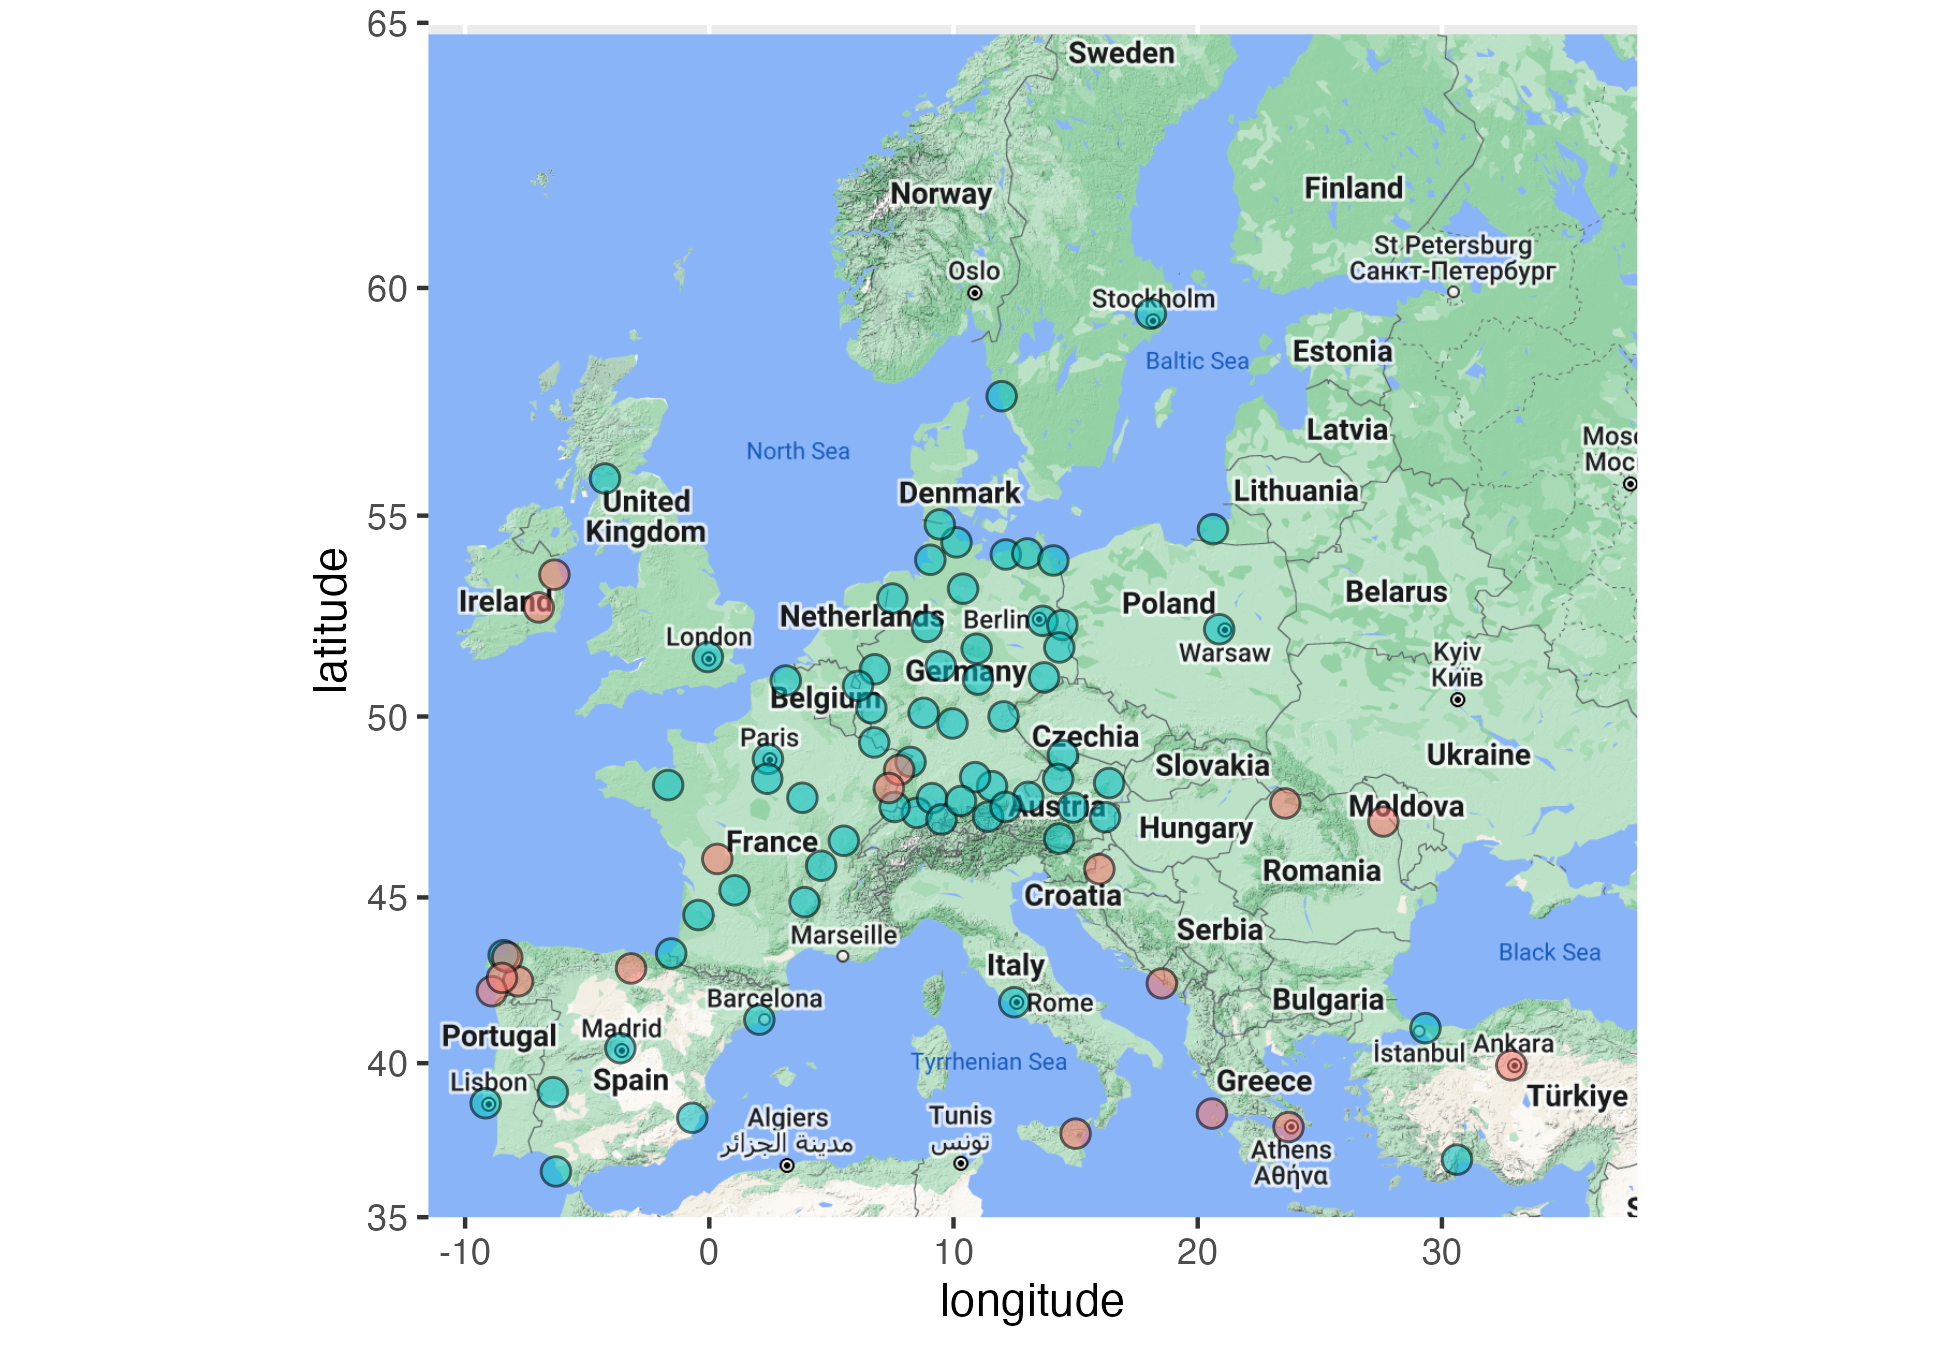
\includegraphics[width=1\linewidth]{../output/plots/map} \caption{Geographical distribution of water analysis reports included in the source water dataset. Green: analysis of municipal tap water (n = 71); Red: rainwater analysis (n = 18).}\label{fig:map}
\end{figure}

\hypertarget{assumptions}{%
\subsection{Assumptions}\label{assumptions}}

The following assumptions have been made:

\begin{itemize}
\tightlist
\item
  the feed input was standardised to \SI{1}{\kg}
\item
  feed nutrient levels based on metadata (commercial and experimental
  fish feeds; n \textgreater{} 50 for N, P; n \textless{} 10 for all
  other elements)
\item
  three nutrient retention levels; means according to Roy et al., 2022
  (TILAFeed), Sugiura et al., 2018, ±5\%
\item
  water nutrient compositions based on metadata (water analysis reports;
  n \textgreater{} 50 for most elements)
\item
  makeup water 10, 100, and 1000 L per kg of feed input (Kloas et al.,
  2015, Dalsgaard et al., 2013)
\item
  at a feeding rate of 2\% BW/day, the resulting biomass of the stock
  from 1 kg feed input is 50 kg
\item
  at a stocking density of 50 kg/1000 L, this results in a system of
  1000 L
\item
  considering the makeup water input, this would correspond to water
  exchange rates of 1\%, 10\%, and 100\%.
\end{itemize}

\hypertarget{outcomes}{%
\subsection{Outcomes}\label{outcomes}}

Figure 2 and 3 show the results of the permutation analysis of tap water
in form of a density plot and an empirical cumulative distribution
function (ECDF).

\begin{figure}
\includegraphics[width=1\linewidth]{../output/plots/permutation_tap_density} \caption{Permutation analysis of the percentage contribution of tap water to the net nutrient input at different makeup water levels (10, 100, and 1000 L/kg of feed input). The density plots visually display the probability density function of the percentage contribution of tap water to the total daily nutrient input, illustrating the likelihood of observing different values. Dashed line marks the 95\% percentil, while the solid line marks the median of the data.}\label{fig:permutation_rain}
\end{figure}

\begin{figure}
\includegraphics[width=1\linewidth]{../output/plots/permutation_tap_ecdf} \caption{Empirical cumulative distribution functions of the percentage contribution of tap water to the net nutrient input at different makeup water levels (10, 100, and 1000 L/kg of feed input). Dashed line marks the 95\% percentil, while the solid line marks the median of the data. Data is based on permutations.}\label{fig:permutation_tap}
\end{figure}

\textbf{In the following, only the markup water of 100 L/kg of feed is
considered, equaling a water exchange rate of 10\%.}

The permutation analysis of the tap water data clearly shows that tap
water contributes below 10\% of the total inputs of N, P, K, Fe, Cu, and
Zn in 50\% of the cases (everything left from solid vertical line). The
least variability in this picture is found for N and P, with 95\% of the
data being very close to the median value of approx, 10\% contribution
to the total N and P input. K and Zn are slightly more variable, with
contributions ranging up to 25\% and 30\%, respectively. The majority of
those nutrients can thus be assumed to originate from the feed with
almost 100\% probability. Consequently, an increase in the inclusion
rate of those nutrients into aquafeeds will likely result in a similar
response in the ``net nutrient input'', irrespective of where in Europe
this feed is applied.

A different picture emerges for Ca and Mg. Here, the contribution of tap
water was found to be up to 35\% and 50\% of the total nutrient input in
50\% of the cases, respectively, and it went as high as 75\% and 90\% of
the total input in 95\% of all possible combinations. Contributions of
S, Fe, and Cu from tap water are relatively low, ranging between 2\% and
12.5\% of the total input in 50\% of the cases. Though, the S input from
tap water can result in up to 50\% of the total input, while it was
found that around 80\% of Fe and Cu can enter the system via the tap
water.

The variability in the results can be partly traced back to the
variability found in the aquafeeds, but also to the high variability in
element concentrations found in the water. It is thus not meaningful to
consider those nutrients for inclusion into specialty feeds, because the
resulting response in nutrient levels will not depend on the nutrients
supplied via feed in all cases, but also on those that are entering the
system via the water. Management strategies for the nutrients mentioned
must therefore probably be adapted to the specific conditions of a
plant, as a generalised overall solution will almost always be the worse
compromise.

\hypertarget{questionssuggestions}{%
\subsection{Questions/Suggestions}\label{questionssuggestions}}

\begin{itemize}
\tightlist
\item
  \textbf{Suggestion:} Focussing on 100 L/kg of feed (10\% water
  exchange rate) only and making a dynamic plot via RShiny that can be
  linked as supplementary material and hosted on the University website
  or on ShinyApps.io to keep the ``big picture'' clean.
\item
  \textbf{Question:} Which metric can better describe the variability in
  contributions? \emph{Effect size}?
\end{itemize}

\hypertarget{rationale}{%
\subsection{Rationale}\label{rationale}}

The few studies that assess the contribution of different nutrient
sources to aquaculture systems (e.g., Delaide et al., 2017; Strauch et
al., 2018) have several flaws when thinking of integrated aquaculture
systems:

\begin{enumerate}
\def\labelenumi{\arabic{enumi}.}
\tightlist
\item
  They report data from a single set of nutrient inputs that is only
  representative for their particular combination of feed and water
  composition and daily mass flows.
\item
  They do not take into account that the amount of nutrients that is
  available for further use in an integrated system is not the gross
  feed input, but the feed input corrected for the retention of
  nutrients by the fed animals.
\end{enumerate}

Overall, there is considerable variation in the composition of aquafeeds
and water and also in their mass flows (water exchange). It was shown
that African catfish and European eel can be reared under a water
replacement as low as \SI{30}{\liter\per\kg} of feed without impairment
of the feed intake (Mota et al., 2015). Nile tilapia was successfully
reared at a water replacement rate of \SI{100}{\liter\per\kg} of feed
(Kloas et al., 2015). In other species such as Rainbow trout and
Sturgeon, a water replacement rate of \SI{1000}{\liter\per\kg} of feed
is common (Dalsgaard et al., 2013). A single scenario such as in the
studies mentioned initially is thus not representative.

\end{document}
